% 2012 年重庆卷文科第 20 题：直三棱柱 ABC-A1B1C1，D 为 AB 中点。
% 来源 PDF：普通高考/2012/2012重庆文.pdf，第 2 页（印面 724）第 2 栏。
% 投影：screen(x,y,z) = (x + 0.45y, 0.55y + 0.75z)，取 AB=4、CD=√5、高 2√2。
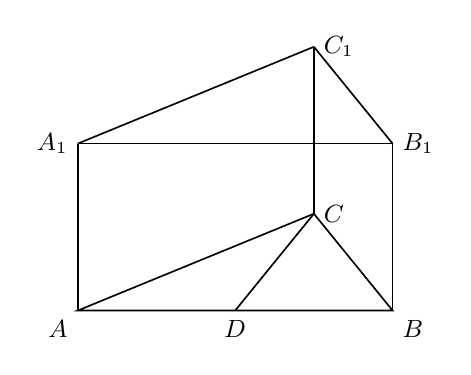
\begin{tikzpicture}[semithick, font=\small]
  \coordinate (A)  at (-2,0);
  \coordinate (B)  at (2,0);
  \coordinate (C)  at (1.0,1.23);
  \coordinate (D)  at (0,0);
  \coordinate (A1) at (-2,2.12);
  \coordinate (B1) at (2,2.12);
  \coordinate (C1) at (1.0,3.35);
  \draw (A) -- (B) -- (C) -- cycle;
  \draw (A) -- (A1);
  \draw (B) -- (B1);
  \draw (C) -- (C1);
  \draw (A1) -- (B1);
  \draw (B1) -- (C1);
  \draw (A1) -- (C1);
  \draw (C) -- (D);
  \node[below left] at (A) {$A$};
  \node[below right] at (B) {$B$};
  \node[right] at (C) {$C$};
  \node[below] at (D) {$D$};
  \node[left] at (A1) {$A_1$};
  \node[right] at (B1) {$B_1$};
  \node[right] at (C1) {$C_1$};
\end{tikzpicture}
